
\section{Asymmetric Cryptography}

\paragraph{Public Key Encryption (PKE) Scheme}
is a triple $PKE = (KGen, Enc, Dec)$.
\\
$KGen$ generates a key pair $(sk, pk) \in \mathcal{SK} \times \mathcal{PK}$. \\
$Enc$ takes a public key $pk$ and a message $m \in \M \subseteq \setzeroone^*$
and produces a ciphertext $c \in \C \subseteq \setzeroone^*$. \\
$Dec$ takes a private key $sk$ and a ciphertext and produces a message or an error $\bot$.
\\
For correctness, we require that $Dec_{sk}( Enc_{pk}(m) ) = m$ (for all keypairs output by $KGen$).

\paragraph{Key distribution}
PKE translates the problem of securely distributing secret symmetric keys into
distributing authentic public keys.

\paragraph{IND-CCA Security}
The adversary gets access to a LoR encryption and a decryption oracle and needs to
distinguish whether the left or the right messages are being encrypted
(see \autoref{fig:pke-ind-cca}).
Compare this with the symmetric game (given in \autoref{fig:ind-cca}).
\\
IND-CPA security is defined the same, but without the decryption oracle.

\begin{figure}[h]
    \centering
	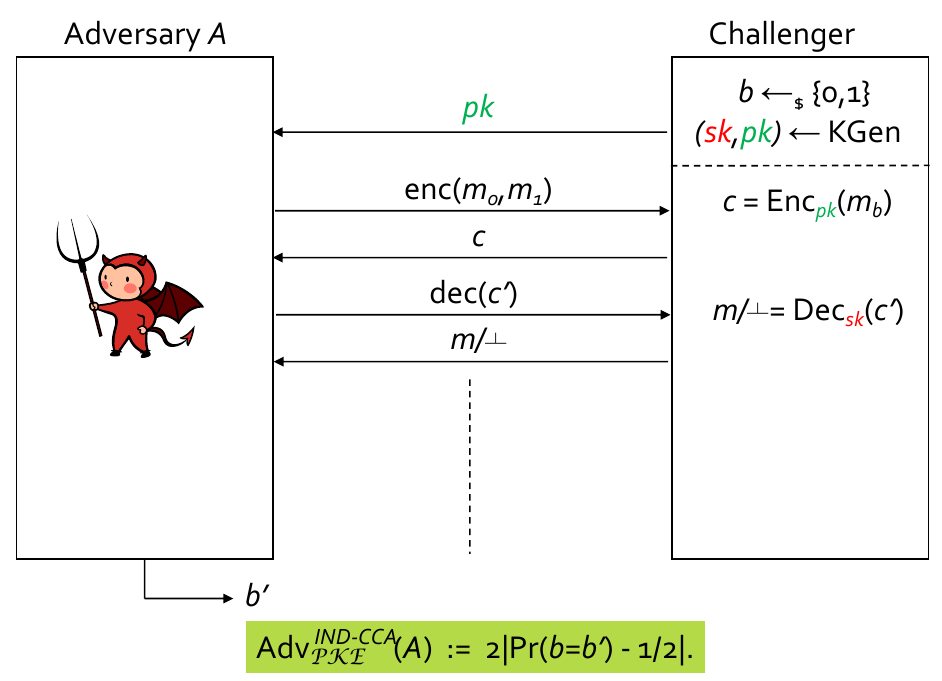
\includegraphics[scale=0.4]{images/pke-ind-cca.png}
    \caption{IND-CCA game for PKE}
    \label{fig:pke-ind-cca}
\end{figure}

\paragraph{Integrity for PKE}
Defining integrity does not make sense in a PKE setting.
Anybody can choose a message, encrypt it under the public key and can thus come
up with a valid ciphertext that will be accepted by the receiver.


\subsection{KEM/DEM Paradigm}

\paragraph{Hybrid encryption}
Asymmetric crypto is expensive (e.g. due to large key sizes).
Idea: encrypt the message symmetrically and encrypt the symmetric key using PKE.

\paragraph{Key Encapsulation Mechanism KEM}
is a triple $(KGen, Encap, Decap)$.
\\
$KGen$ generates a random key pair $(sk, pk)$. \\
$Encap$ takes a public key $pk$ and generates a random key $K$, outputting the encapsulation $c$ and the generated key: $(c, K) \in \C \times \K$. \\
$Decap$ takes a private key $sk$ and an encapsulation $c$ and outputs either the key $K$ or an error $\bot$.
\\
For correctness, we require that if $(c, K) \leftarrow Encap(pk)$ then $K \leftarrow Decap(sk, c)$.

Note that unlike PKE, $Encap$ has no message input.
Instead, it internally generates a key.

\paragraph{IND-CCA Security for KEMs}
The adversary needs to distinguish between an encapsulated key $K_0$
(for which it gets the encapsulation $c$) and a randomly generated key $K_1$.
See \autoref{fig:kem-ind-cca}.

\begin{figure}[h]
    \centering
	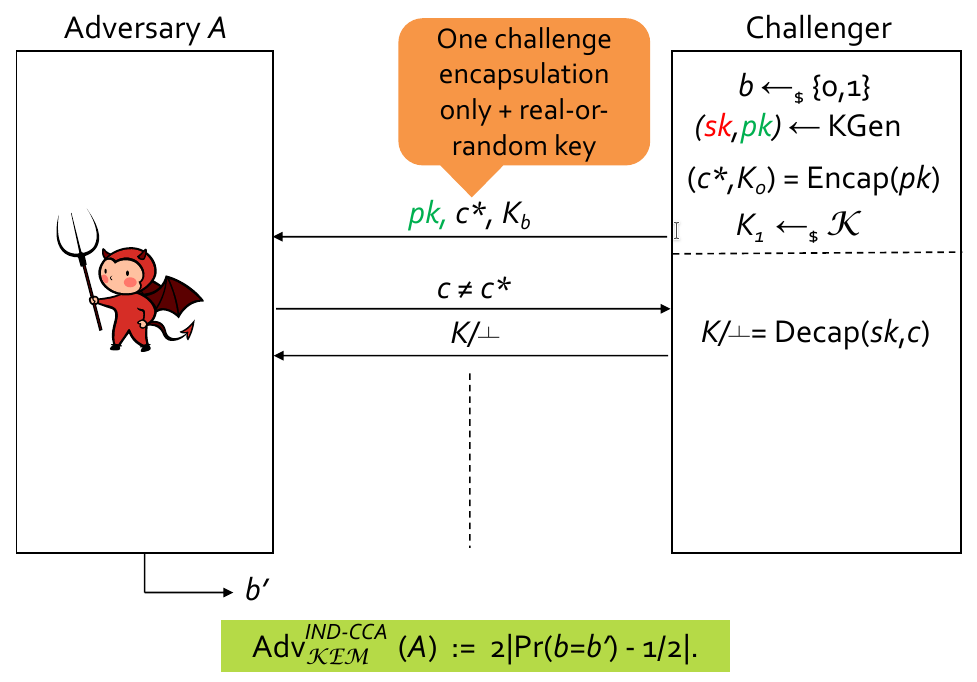
\includegraphics[scale=0.4]{images/kem-ind-cca.png}
    \caption{IND-CCA game for KEM}
    \label{fig:kem-ind-cca}
\end{figure}

\paragraph{Data Encapsulation Mechanism DEM}
is simply a symmetric encryption scheme.

\paragraph{KEM/DEM Composition Paradigm}
We can build a PKE scheme from a KEM and a DEM:
\\
$PKE.KGen$:
$(sk, pk) = KEM.KGen()$; return $(sk, pk)$
\\
$PKE.Enc$:
$(c_0, K) = KEM.Encap(pk)$; $c_1 = DEM.Enc(K, m)$; return $(c_0, c_1)$
\\
$PKE.Dec$:
$m = \bot$; $K = KEM.Decap(sk, c_0)$; if $K \neq \bot$ then $m = DEM.Dec(K, c_1)$; return $m$

Theorem: If both KEM and DEM are IND-CCA secure, then so is the composed PKE.
The proof proceeds using game hopping.


\subsection{RSA}

\paragraph{Textbook RSA}\mbox{}\\
$KGen$:
Generates random primes $p, q$ of size $\frac{k}{2}$ bits.
Sets $N=pq$.
Also generates integers $d, e$ such that $de = 1 \mod (p-1)(q-1)$.
Outputs keypair $(sk, pk)$ s.t. $sk = d$ and $pk = (e, N)$.
\\
$Enc$:
Outputs $c = m^e \mod N$.
\\
$Dec$:
Outputs $m = c^d \mod N$.

\textbf{NOT secure}.
Not randomised, so cannot satisfy IND-CPA.
Also malleable: $(m_0 \cdot m_1)^e = m_0^e \cdot m_1^e $.

Questions:
How to generate $p, q, d, e$?
How to encode messages as integers in $[1, N-1]$?

\paragraph{Generating keys}
Needs a good source of randomness and primality test.
Things can still go wrong:
shared prime factors\footnote{See ``Mining your p's and q's.''},
over-optimised prime generation, bad primality tests.

From $e$, $d$ can be calculated using the Extended Euclidean algorithm (knowing $p, q$).
In practice, $e = 2^{16}+1 = 65537$ is often used for faster encryption (prime + likely coprime to $(p-1)(q-1)$).

Other optimisations lead to vulnerabilities:
\begin{itemize}
\item Small $e$:
If $e$ is small (e.g. $e=3$), then for small messages it can happen that $c=m^3$ holds over the integers, i.e. without modular reduction.
Then an attacker can simply take the (cube) root to recover $m$.
\item Small $d$:
insecure up for $d \leq N^{1/4}$ (Weiner's attack)
\end{itemize}

\paragraph{Keysize requirements}
By breaking the \emph{Integer Factorisation Problem (IFP)} (to factor $N$) we can break RSA (the reverse may not hold!).
One algorithm for the IFP is the \emph{Number Field Sieve (NFS)}.
Generally, the best known algorithms are super-polynomial, but sub-exponential.

See \href{https://www.keylength.com/}{keylength.com} for key size recommendations.

\paragraph{Malleability}
Since textbook RSA is malleable, an attacker can choose an arbitrary $s$ and amend the message:
$s^e \cdot c \mod N$ decrypts to $s \cdot m \mod N$.

\paragraph{Padding}
Goals:
introduce randomness,
expand short messages to full size,
and destroy algebraic relationship (removing malleability property)
to achieve IND-CCA security.

\paragraph{PKCS\#1 v1.5 Padding}
Structure:
Two most significant bytes set to \mbox{\texttt{0x00 0x02}},
then $\geq 8$ random non-zero bytes,
then a zero byte and finally the message $m$ as the left most bytes.
Implies a maximum message size of $k-11$ bytes (assuming $N$ as $k$ bytes).

Encryption: $pad(m)^e \mod N$ \\
Decryption: $m' = c^d \mod N$, then check for correct padding and return $m$.

\underline{Not} IND-CCA secure.

\begin{figure}[h]
    \centering
	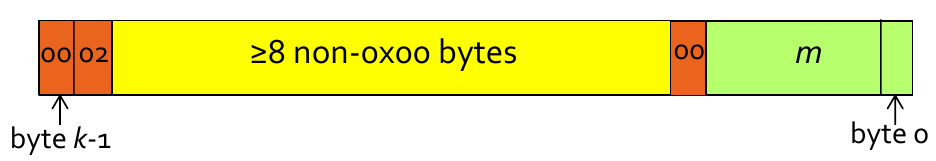
\includegraphics[scale=0.4]{images/rsa-pkcs.png}
    \caption{PKCS\#1 v1.5 Padding}
    \label{fig:rsa-pkcs}
\end{figure}

\paragraph{Bleichenbacher's Attack on PKCS\#1 v1.5}
Let $m' = (00\ 02\ ||\ r\ ||\ 00\ ||\ m)$ be the encoded message and let $c = m'^e \mod N$.
Attacker asks oracle to decrypt $s^e \cdot c \mod N$.
With probability $\approx 2^{-16}$ the padding is valid and decryption does not return a padding error.
\\
Through an \emph{adaptive attack}, using carefully chosen $s$, one can eventually recover $m'$ (and thus $m$).

Originally this required around $2^{20}$ queries but has since improved to 5-10K queries for a 1024 bit modulus.
For attacks against TLS, see \href{https://drownattack.com/}{DROWN} and \href{https://robotattack.org/}{ROBOT}.

\paragraph{RSA-OAEP Padding}
Optimal Asymmetric Encryption Padding, standardised in PKCS\#1 v2.1, yet not as widely adopted.

Setup:
Let $n$ be the bitsize of $N$.
Let $k_0, k_1$ be such that no adversary can perform neither $2^{k_0}$ nor $2^{k_1}$ operations in reasonable time (e.g. 128).
Messages are assumed to be bitstrings of length $n - k_0 - k_1$.
Let $G, H$ be hash functions such that
$G: \setzeroone^{k_0} \mapsto \setzeroone^{n-k_0}$
and $H: \setzeroone^{n-k_0} \mapsto \setzeroone^{k_0}$.

Encoding:
See \autoref{fig:rsa-oaep}.
At the end, compute $c = (X\ ||\ Y)^e \mod N$.

Decoding:
decrypt, then reverse the encoding, then check for the presence of the zero bits.

Can be proven to be IND-CCA secure (under strong number theoretic assumptions, including the Random Oracle Model).
Intuition: output of hash functions is random, breaking up any algebraic relationships.

\begin{figure}[h]
    \centering
	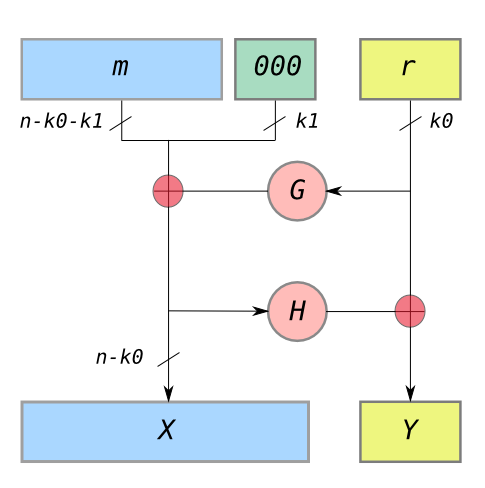
\includegraphics[scale=0.45]{images/rsa-oaep.png}
    \caption{RSA-OAEP Padding}
    \label{fig:rsa-oaep}
\end{figure}

\paragraph{Random Oracle Model ROM}
Strong abstraction of hash functions: models hash functions as truly random functions.

A practical problem for proofs is that evaluating a random function can take exponential time -- but we only consider poly-time adversaries!
We solve this by ``stopping time'' when the adversary invokes a hash function,
and forcing the adversary to use an oracle to evaluate the hash function for them.
This extra oracle can inspect the adversary's queries, sample new random values for fresh queries, and return the values for repeated queries from its cache.

\paragraph{RSA (Inversion) Problem}
Summarizes the task of performing an RSA private-key operation given only the public key.
Specifically for decryption, the task is to compute $m$ given only $c$ and $(e, N)$.

One -- but not the only -- way to solve this is by factoring $N$.
There is no proof that the IFP or the RSA problem are (computationally) hard.
The RSA problem is at least as easy as the IFP, but it might be easier.
(Finding $d$ is equivalent to factoring though.)


\subsection{Discrete Logarithm / Diffie-Hellman}

\paragraph{Discrete Logarithm Setting}
Let $p, q$ be large primes such that $q$ divides $p-1$, i.e. $p = kq + 1$.
Now choose a random $h$ and compute $g = h^{(p-1)/q} \mod p$ (repeat until $g \neq 1$).
Observations:
\begin{itemize}
\item
If $g \neq 1$ then the $q$ powers of $g$ -- namely $G_q = \{ g, g^2, g^3, \dots, g^q \}$
-- are all distinct mod $p$.
\item
$g^q = 1 \mod p$
\item
Multiplying any two elements of $G_q$ results in another element of $G_q$.
\end{itemize}
Together, this means that $G_q$ forms a \emph{group} under multiplication mod $p$.
In particular, $G_q$ is a cyclic group with generator $g$ and prime order $q$ (number of group elements).

\paragraph{Discrete Logarithm Problem DLP}
Let $G_q$ be a cyclic group with generator $g$ and prime order $q$.
Set $y = g^x \mod p$ where $x$ is uniformly random in $\{ 0, 1, \dots , q-1 \}$\footnote{Note that $g^0 = 1 = g^q$.}.
The task is to find $x$.

Algorithms to solve the DLP include the \emph{Function Field Sieve}
(sub-exponential but super-polynomial in $\log p$) or
the \emph{Pollard-$\rho$ Algorithm} (exponential in $\log q$).


\paragraph{Diffie-Hellman Key Exchange DHKE}
The group and $(p, q, q)$ are public parameters.
Alice picks a random $x$ and sends $X = g^x \mod p$ to Bob.
Bob picks a random $y$ and sends $Y = g^y \mod p$ to Alice.
Both compute a shared key $K = Y^x = X^y = g^{xy} \mod p$.

This is the modern view of the dynamic DHKE, where the private values $x, y$ are considered \emph{ephemeral} and are generated freshly each time.
In the original paper the key exchange was static -- participants would upload their key share to public, authentic directory.
\\
Furthermore in applications we don't usually use $K$ directly but use a KDF to derive keys from it.

Note that this is NOT yet public-key encryption!

\paragraph{MITM Attack on DHKE}
An active MITM attacker can trivially run two DHKEs with both parties and relay messages,
thus completely compromising the security of the ``modern'' interactive DHKE.
\\
As a countermeasure, we need to provide authenticity of the public key shares.
This can be done either using MACs (requires a pre-shared symmetric key -- but DHKE still gives forward secrecy)
or using signatures (requires a PKI).

\paragraph{Computational Diffie-Hellman Problem CDHP}
Given $(p, q, q)$ and $g^a \mod p$ and $g^b \mod p$ find $g^{ab} \mod p$.

There is no proof that CDHP is equivalent to DLP (it could be easier), but is believed to be equivalent.

\paragraph{Decisional Diffie-Hellman Problem DDHP}
Given $(p, q, q)$ and u.a.r. values $a, b, c$ distinguish between
$(g^a, g^b, g^{ab})$ (a \emph{DDH triplet}) and $(g^a, g^b, g^c)$.

It is believed that the DDH assumption is stronger than the discrete logarithm assumption,
because there exist cyclic groups where the DLP is hard but the DDHP is easy.
 

\paragraph{ElGamal PKE scheme}
Public group parameters $(p, q, g)$.
\\
$KGen$:
Choose $x \leftarrow \$ \{ 0, 1, \dots, q-1 \}$ u.a.r.\footnote{$\leftarrow\$$ denotes drawing at random.}.
Set $sk = x, pk = X = g^x \mod p$.
\\
$Enc$:
Choose $r \leftarrow \$ \{ 0, 1, \dots, q-1 \}$ u.a.r. and set $Y = g^r \mod p$.
Compute $Z = X^r \mod p$.
Compute $C' = M \cdot Z \mod p$.
Output ciphertext $C = (Y, C')$.
\\
$Dec$:
Check that $Y \in G_q$ (else return $\bot$)\footnote{There are attacks if $Y \not \in G_q$.}.
Compute $Z' = Y^x \mod p$.
Output $M = C' \cdot (Z')^{-1} \mod p$.
\\
Correctness: left as an exercise.

Intuition: combine a long-term and a one-time key share.
Use the resulting DH value $Z$ as an encryption mask.

IND-CPA secure under the DDH assumption. \\
NOT IND-CCA secure (find an attack!).


\paragraph{Diffie-Hellman Integrated Encryption Scheme DHIES} \mbox{} \\
Motivation:
Addresses ElGamal's problems: missing IND-CCA and having to encode messages as group elements.

Definition:
Public parameters $(p,q,g)$ and a hash function $H$ with a suitable output domain.
\\
$KGen$:
Choose $x \leftarrow \$ \{ 0, 1, \dots, q-1 \}$ u.a.r..
Set $sk = x, pk = X = g^x \mod p$.
\\
$Enc$:
Choose $r \leftarrow \$ \{ 0, 1, \dots, q-1 \}$ u.a.r. and set $Y = g^r \mod p$.
Compute $Z = X^r \mod p$.
Set $K = H(Z, X, Y) = K_e\ ||\ K_m$.
Compute $C' = EtM(M)$ using $K_e, K_m$ as encryption and MAC keys.
Output $C=(Y, C')$.
\\
$Dec$:
Check that $Y \in G_q$ (else return $\bot$).
Compute $Z' = Y^x \mod p$.
Recompute $K$ and decrypt.

Intuition: effectively a KEM/DEM construction. Can plug in any AE scheme.

IND-CCA secure in the Random Oracle Model.


\subsection{Signatures}

\paragraph{Signature scheme}
Goal: provide integrity. Public key analogue of MAC schemes.

$KGen$: generates a random key pair $(sk, vk)$ = (signing key, verification key)
\\
$Sign$: takes an input a signing key $sk$ and a message $m$ and outputs the signature $\sigma$
\\
$Vfy$: takes as an input $(vk, m, \sigma)$ and outputs 0 or 1%
\footnote{Some schemes perform ``message recovery'': they recover $m$ from $\sigma$ rather than receiving $m$ as input.}.
\\
Correctness:
for all $(sk, pk)$ produced by $KGen$\footnote{Notice that this definition says nothing about maliciously generated key pairs.}
and for all $m \in \setzeroone^*$ if $\sigma = Sign(sk, m)$ then $Vfy(vk, m, \sigma) = 1$.

\paragraph{UF-CMA Security}
We define \emph{(Existential) Unforgeability under Chosen Message Attack (E)UF-CMA}
through the security game given in \autoref{fig:uf-cma}.
We give the adversary access to $vk$ and a signing oracle.

Informally: it should be hard for an adversary to produce a valid signature for a \underline{fresh} message $m^*$.
\\
Formally:
The adversary wins if $m^*$ is distinct from all queried $m$ and $Vfy(vk, m^*, \sigma^*) = 1$.

Implication: if $vk$ is bound to an identity, one cannot deny having signed $m$ (\emph{non-repudiation})\footnote{Can MACs offer this?}.

\begin{figure}[h]
    \centering
	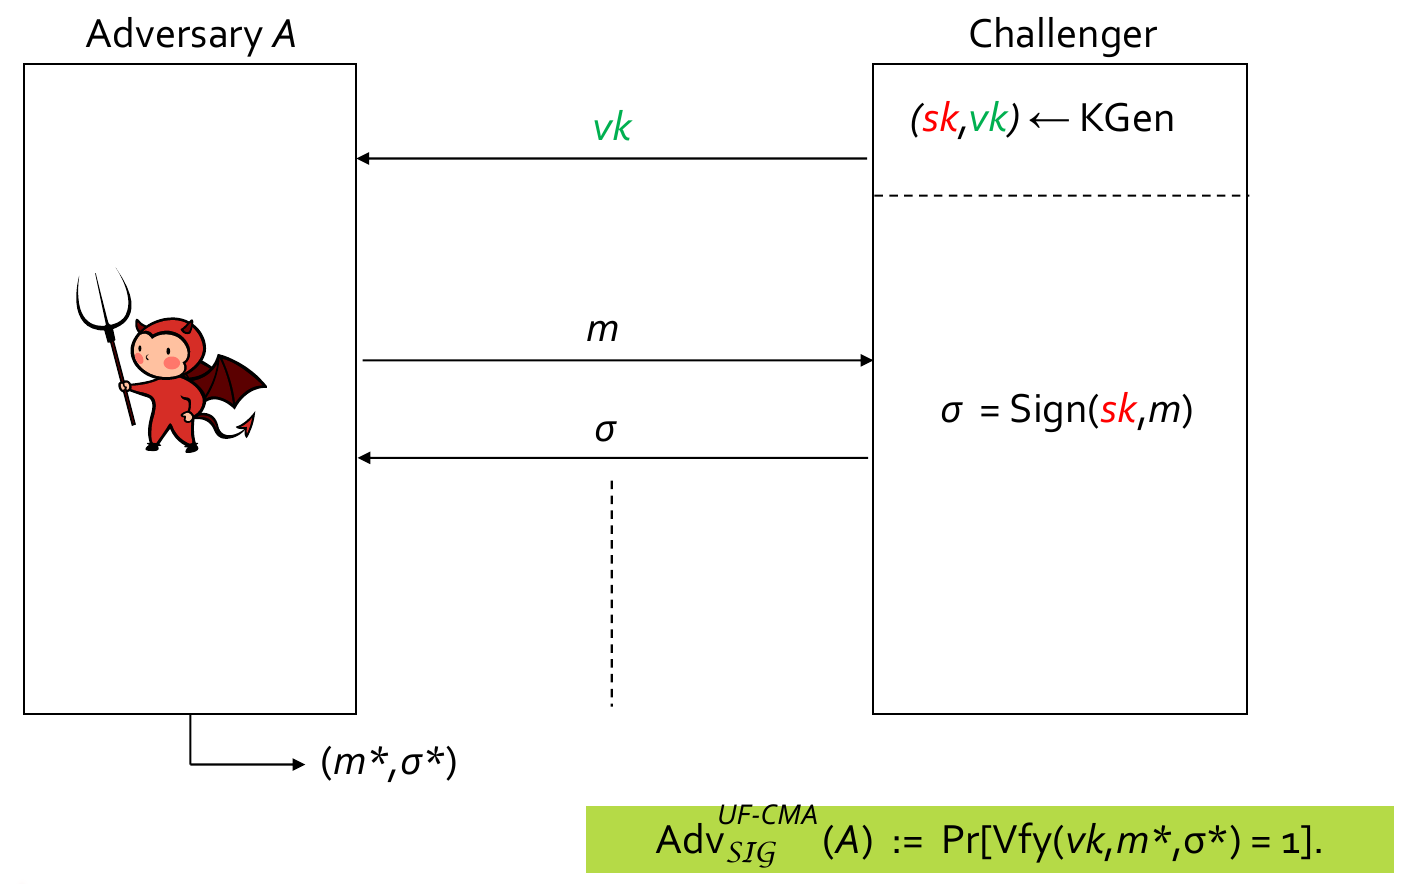
\includegraphics[scale=0.35]{images/uf-cma.png}
    \caption{UF-CMA game}
    \label{fig:uf-cma}
\end{figure}

\paragraph{SUF-CMA Security}
Strong unforgeability: same game as UF-CMA.

Informally:
it should be hard for an adversary to produce a \underline{fresh} valid signature for a \underline{some} message $m^*$.
\\
Formally:
The adversary wins if $(m^*, \sigma^*)$ is distinct from all queried pairs $(m, \sigma)$ and $Vfy(vk, m^*, \sigma^*) = 1$.

We give the adversary more power: they can also win by producing a new signature on a previously queried message.
Note that SUF-CMA and UF-CMA are equivalent for schemes with unique signatures.

\paragraph{Digital Signature Algorithm DSA}
DLP-based, public parameters $(p,q,g)$.

$KGen$: Choose random $sk = x$ and compute $vk = X = g^x \mod p$.
\\
$Sign$:
\begin{enumerate}
\item Generate a random $k \in \{1, ..., q-1\}$
\item Compute $r = (g^k \mod p) \mod q$
\item Compute $k^{-1} \mod q$ and hash $H(m)$
\item Compute $s = k^{-1} \cdot (H(m) + x \cdot r) \mod q$
\item Output $\sigma = (r, s)$
\end{enumerate}
%
$Vfy$:
\begin{enumerate}
\item Check that $r, s \in \{1, ..., q-1\}$
\item Compute $w = s^{-1} \mod q$
\item Compute $u_1 = w \cdot H(m) \mod q$ and $u_2 = w \cdot r \mod q$
\item Output 1 if $(g^{u_1} X^{u_2} \mod p) \mod q = r$ else 0
\end{enumerate}
%
Correctness: left as an exercise.

\paragraph{DSA Security}
Informally:
A hash collision results in a forgery. Usual DLP attack on $sk$.
\\
Formally:
No good security proof for DSA is known.

\emph{Catastrophic failure} under randomness failure:
\\
Assume the same $k$ is used to sign two different messages.
This is detectable since then $r_1 = r_2$.
This knowledge allows to rearrange the two formulas, recover $k$ and solve for $sk=x$!
\\
This issue is real: OpenSSL 2008, PlayStation 2010, Android 2013, any virtualized environment.
\\
We can \emph{hedge} against this by \emph{derandomising}:
generate pseudo-random $k=F_K(vk||m$). Need to keep the PRF key $K$ together with $sk$.

\paragraph{Naïve RSA signature}
Sign using $\sigma = m^d \mod N$.
Verify by $\sigma^e \overset{?}{=} m \mod N$.

INSECURE.
Trivial forgery: $\sigma_1 \sigma_2 \mod N$ is a signature on $m_1 m_2$.

\paragraph{Full-Domain Hash (FDH) RSA signature}
Sign using $\sigma = H(m)^d \mod N$.
Verify by $\sigma^e \overset{?}{=} H(m) \mod N$.

Hash function destroys algebraic (multiplicative) structure.
Allows signing long messages.
But: needs a hash function with the output domain $\{0, ..., N-1\}$.

Theorem:
If the RSA problem is hard and $H$ is a random oracle then FDH is UF-CMA secure.

\paragraph{Hash-based RSA signature with padding}
Sign using $\sigma = pad(H(m))^d \mod N$ for some padding function $pad$.
Verify by $\sigma^e \overset{?}{=} pad(H(m)) \mod N$.

Relaxes requirement of hash function having a matching output domain.
Used e.g. in PKCS\#1 v1.5 with padding $00\ 01\ FF\ ...\ FF\ ||\ c\ ||\ H(m)$ for constant $c$.
\\
Bleichenbacher applies (if padding oracle in implementation).
No known security proof for scheme with PKCS\#1 v1.5 padding.

\paragraph{RSA Probabilistic Signature Scheme RSA-PSS}
See \autoref{fig:rsa-pss} where $H, G_1, G_2$ are hash functions with suitable output lengths.
\\
Sign using $\sigma = (0 || s || t || u)^d \mod N$.
Verify by $(b || s' || t' || u') = \sigma^e \mod N$,
computing $r' = G_1(s') \xor t'$ and then re-encoding from the start and checking for a match.

Standardised e.g. in PKCS\#1 v2.1.

Theorem:
If $H, G_1, G_2$ are random oracles then the UF-CMA security of RSA-PSS is
\underline{tightly} related to the hardness of the RSA problem.

\begin{figure}[h]
    \centering
	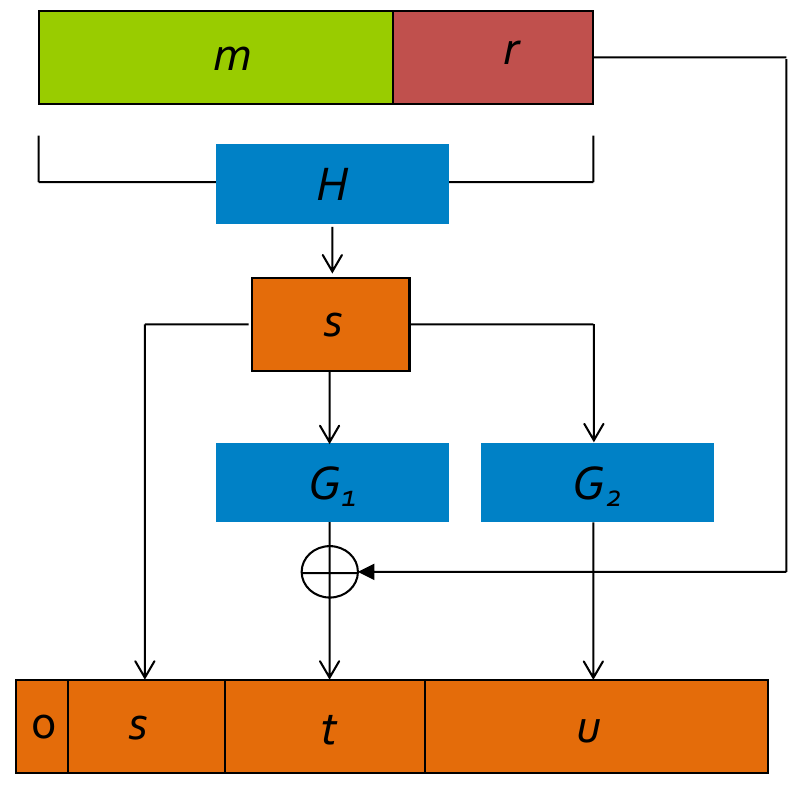
\includegraphics[scale=0.3]{images/rsa-pss.png}
    \caption{RSA-PSS}
    \label{fig:rsa-pss}
\end{figure}

